\subsection{Suprising Symmedian}

Interestingly, the Symmedian Point $X_6$ is the only triangular center out of Kimberling's first 12 whose locus is non-elliptic, though just by a smidgen: for an $a=1.5$ Billiard, the average error with respect to the best fit ellipse is of the order of $10^{-4}$, i.e., imperceptible to the naked eye. Figure~\ref{fig:symmedian} shows the locus of $X_6$ with the deviation from a perfect ellipse exaggerated a million-fold. In fact \cite{ronaldo19a}:

\begin{observation}
The locus of the Symmedian Point $X_6$ of an $N=3$ orbit is a convex quartic.
\end{observation}

\begin{figure}[H]
    \centering
    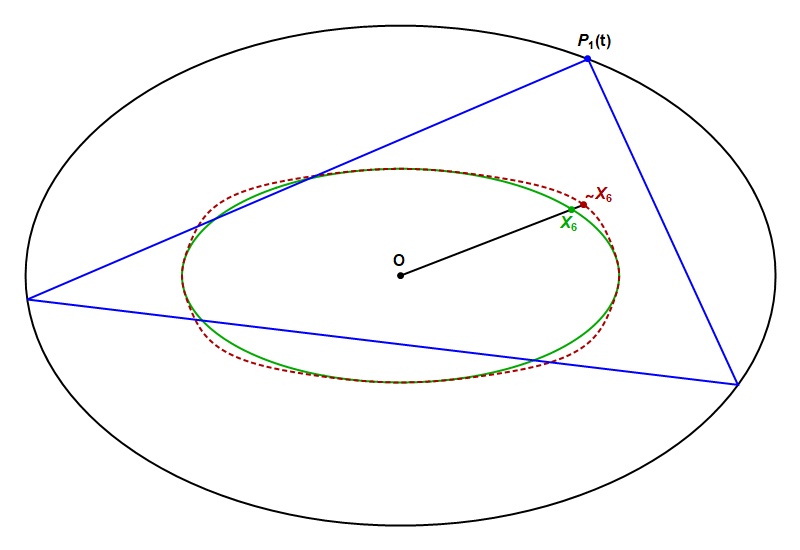
\includegraphics[width=.75\textwidth]{pics/0041_symmedian.png}
    \caption{The convex, quartic locus of the Symmedian Point $X_6$ (green), indistinguishable to the naked eye from an ellipse. The dashed red path shows the locus with the error with respect to a best-fit ellipse exaggerated a million-fold.}
    \label{fig:symmedian}
\end{figure}

\subsection{One Kinky Locus}

The locus of the Orthocenter $X_4$ is elliptic and similar to a rotated copy of the Billiard \cite{ronaldo19a}. At a particular aspect ratio $a_1\simeq{1.51}$, the locus is identical to the Billiard.

Another notable threshold is $a_0\simeq{1.352}$. A choice of $a<a_0$ (resp. $a>a_0$) will result in an orbit family without (resp. with) obtuse triangles, Figure~\ref{fig:orthocenter_loci}. 

\begin{figure}[H]
    \centering
    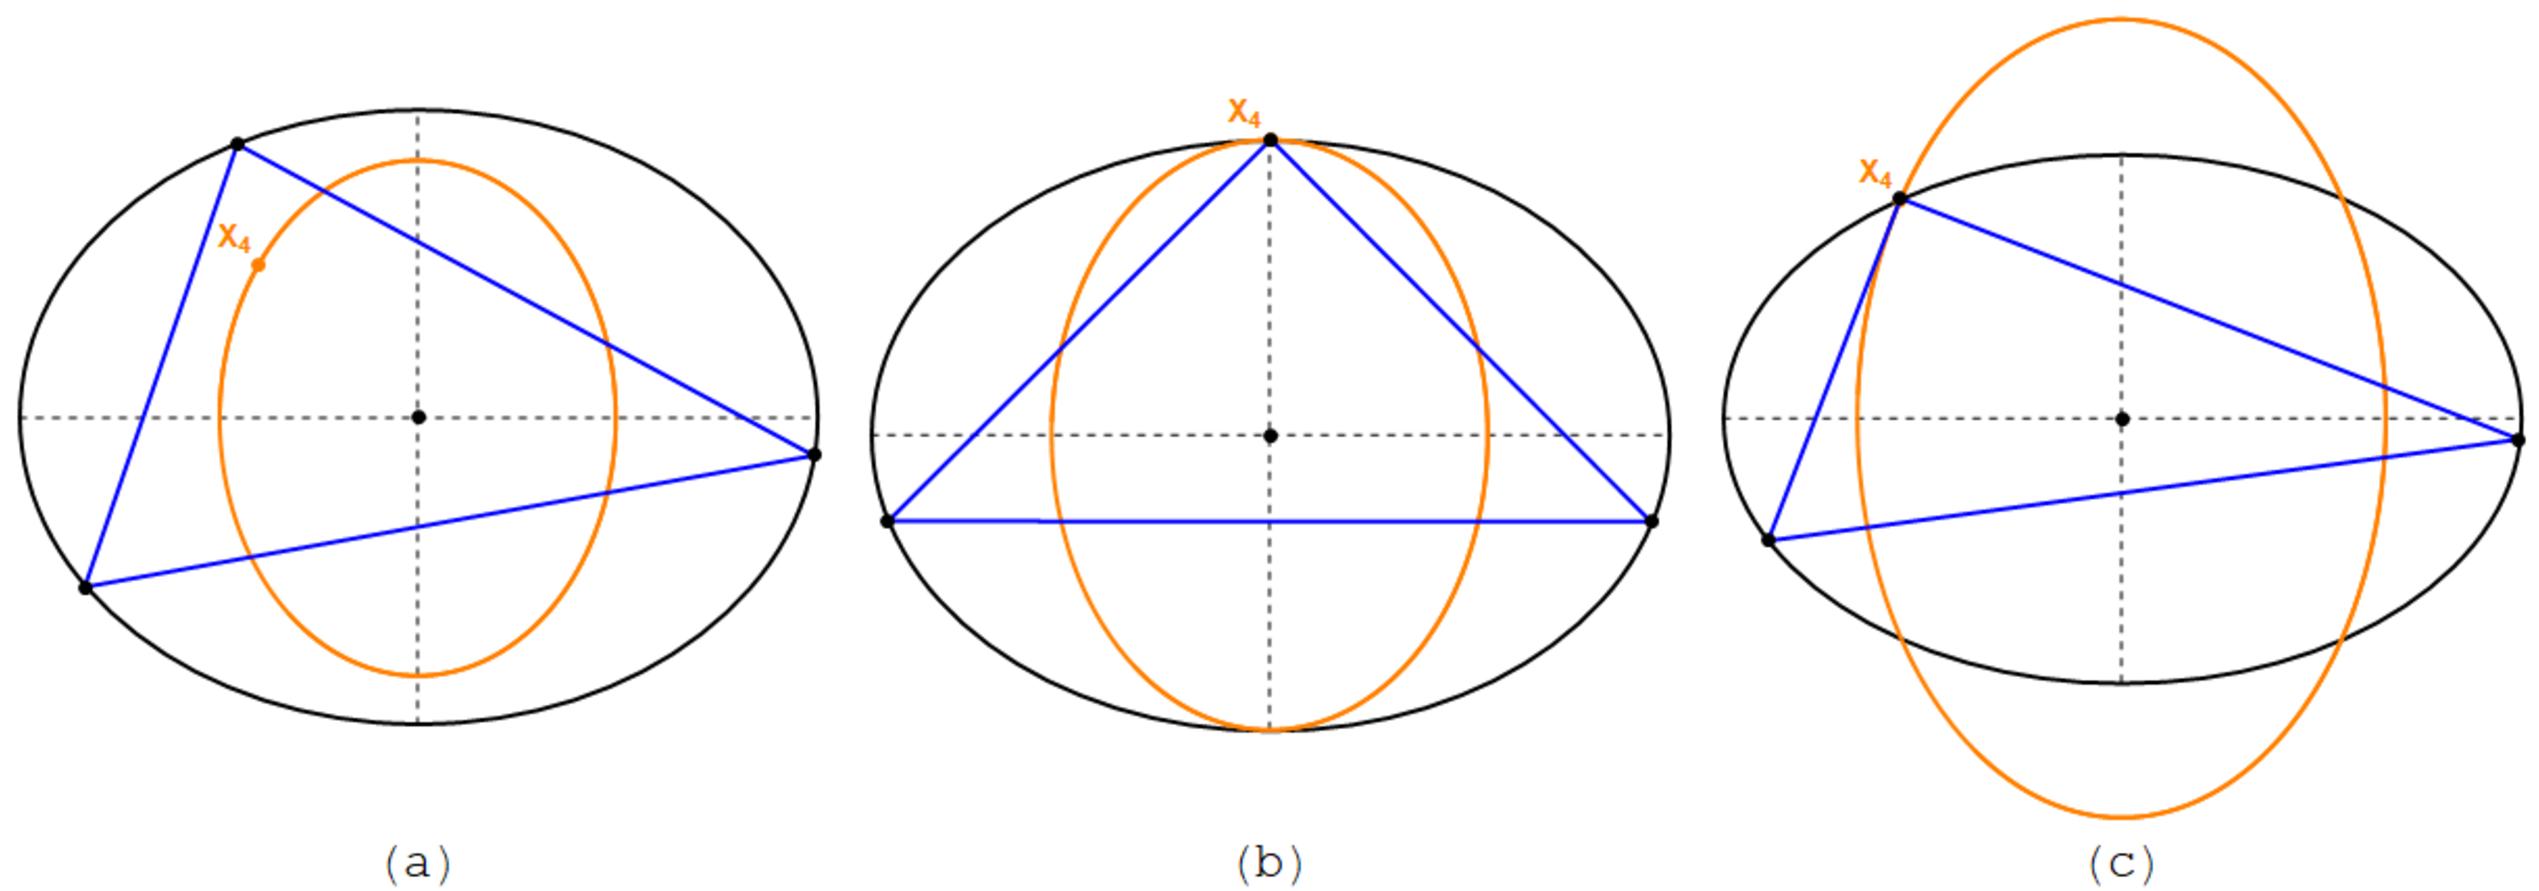
\includegraphics[width=\textwidth]{pics/0045_ort_loci.pdf}
    \caption{Let $B$ be the Billiard (black), $H$ the locus of the orthocenter $X_4$ (orange), and $a_0\simeq{1.352}$. (a) $a<a_0$: $H$  is within $B$ and orbits (blue) can never be obtuse. (b) $a\simeq{a_0}$: $H$ is tangent to $B$ at its top and bottom vertices. An orbit is a right triangle when any of its vertices is at said locations. (c) $a>a_0$: $H$ intersects $B$ on four points. When $X_4$ is inside (resp. outside) $B$, the orbit is acute (resp. obtuse).}
    \label{fig:orthocenter_loci}
\end{figure}

Assume now $a>a_0$ and that $T_h$ is the orbit's {\em Orthic Triangle} \cite{mw}. The Incenter $I_h$ of $T_h$ will display a {\em switching} behavior \cite{coxeter67}:

\begin{center}
\begin{tabular}{r|l}
 orbit & $I_h$ location \\ 
 \hline
 acute & orthocenter $X_4$ \\  
 obtuse & obtuse vertex 
\end{tabular}
\end{center}

At the current choice of aspect ratio, the orbit will be at times acute and obtuse, and the result is the locus of $I_h$ becomes piecewise elliptic, Figure~\ref{fig:orthic_incenter_locus} and \cite[video \#6]{dsr_main_videos_2019}.

\begin{figure}[H]
    \centering
    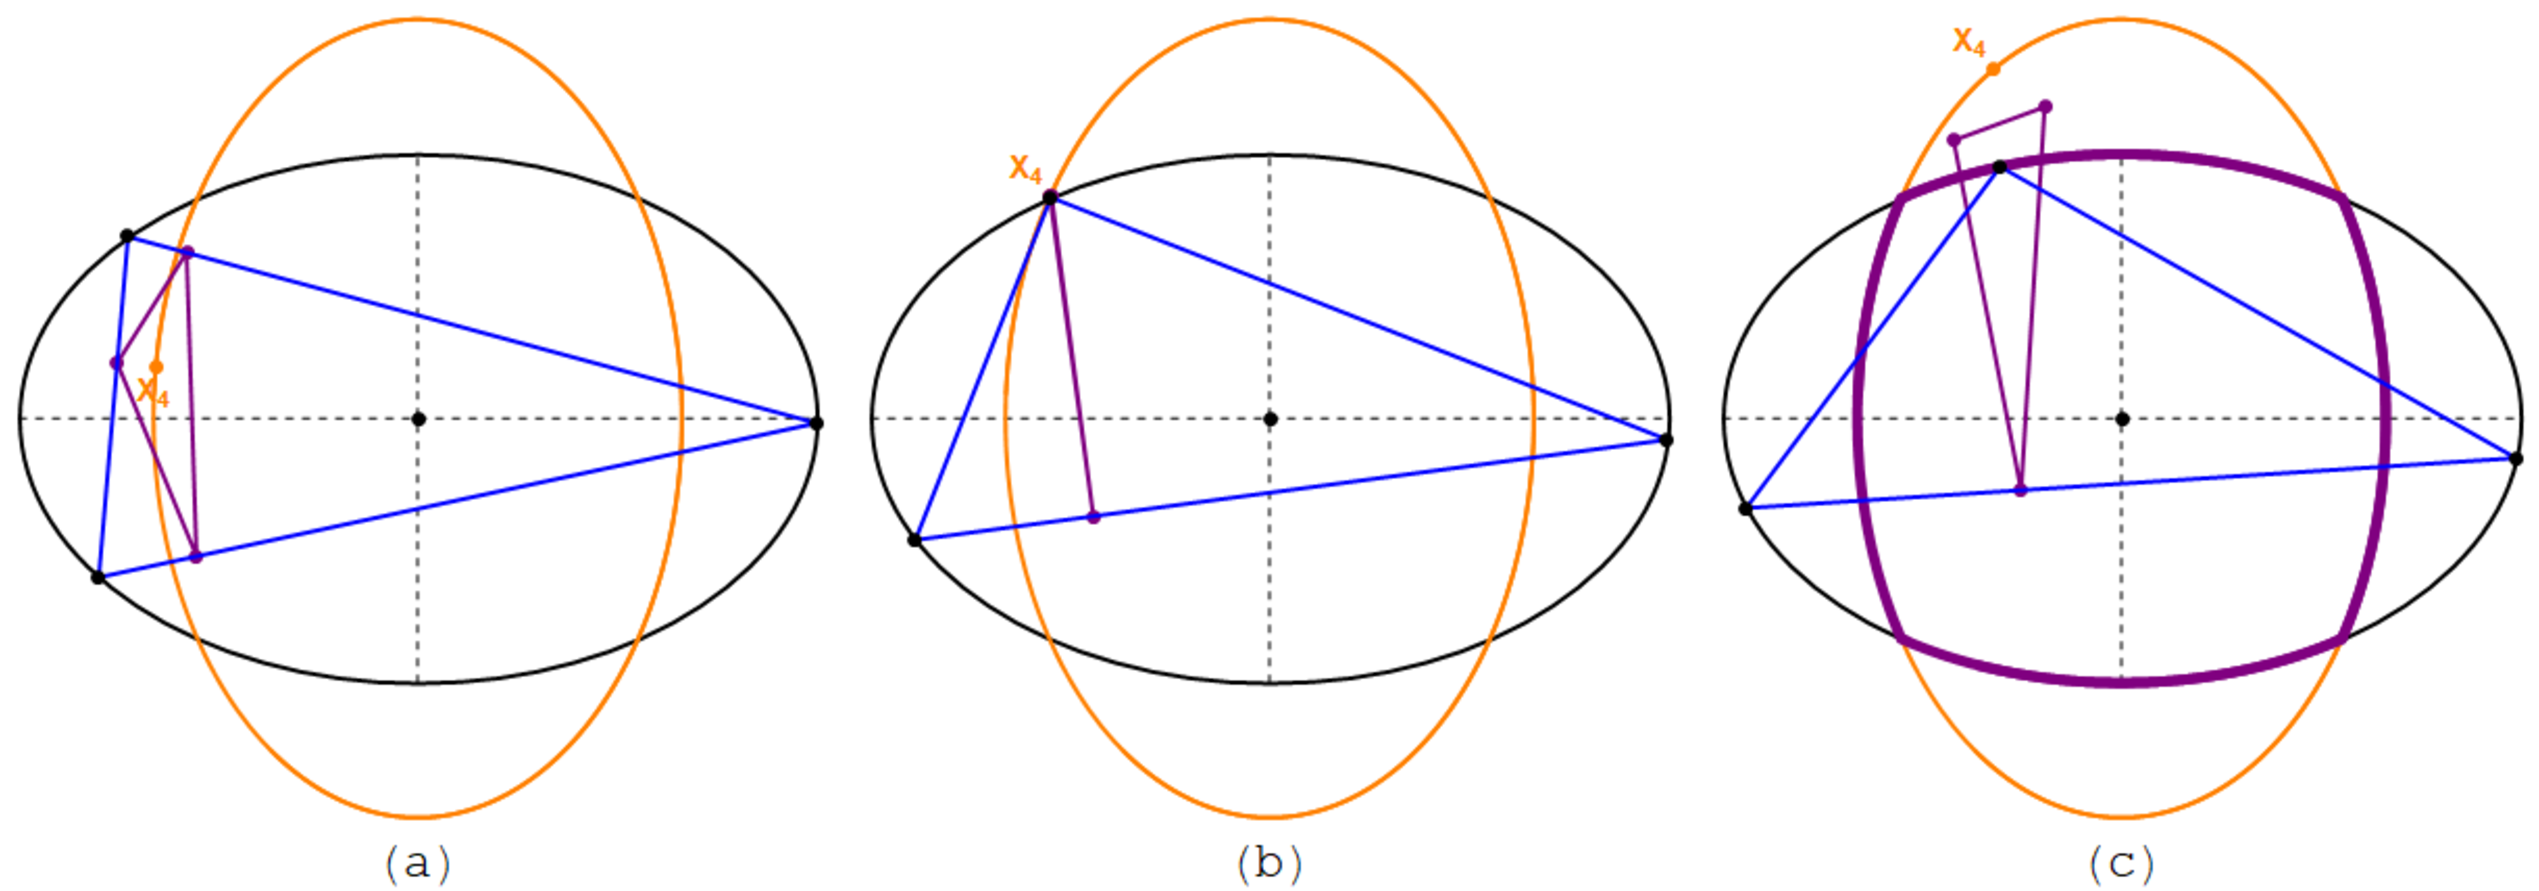
\includegraphics[width=\textwidth]{pics/0045_ort_loci_orthic.pdf}
    \caption{Denote $T$ as an orbit (blue) and $T_h$ its Orthic Triangle (purple). (a) at this orbit position, $X_4$ is inside $B$, $T$ is acute, and $T_h$ is well-conditioned. Its incenter coincides with $X_4$. (b) $X_4$ is now on $B$, $T$ is a right triangle, and $T_h$ degenerates to a segment. (c) $X_4$ lies outside $B$, two of $T_h$'s vertices lie outside $T$. Its incenter separates from $X_4$ and is now congruent with the obtuse vertex. In general, if $a>a_0$, the locus of the Incenter of the Orthic is a four-piecewise-elliptic curve with four kinks.}
    \label{fig:orthic_incenter_locus}
\end{figure}

\begin{observation}
For a Billiard with $a>a_0$ the locus of the Incenter of the orbit's Orthic Triangle is a piecewise-elliptic curve with four kinks.
\end{observation}

\subsection{Complimentary Anticomplementary Phenomena}

Consider the Orbit's Anticomplementary Triangle \cite{mw}, shown in Figure~\ref{fig:act_intouch}. Its own Incircle touches it at three contact points as well as its 9-Point Circle (congruent with the orbit's Circumcircle \cite{mw}) at {\em its} Feuerbach Point. Above it was pointed out the latter's locus is the Billiard. Remarkably:

\begin{observation}
The vertices of the anticomplementary's Intouch Triangle sweep the Billiard.
\end{observation}

\noindent This phenomenon can be viewed here \cite[video \#7]{dsr_main_videos_2019} and proof has been kindly contributed \cite{minevich17,minevich19}.

\begin{figure}[H]
    \centering
    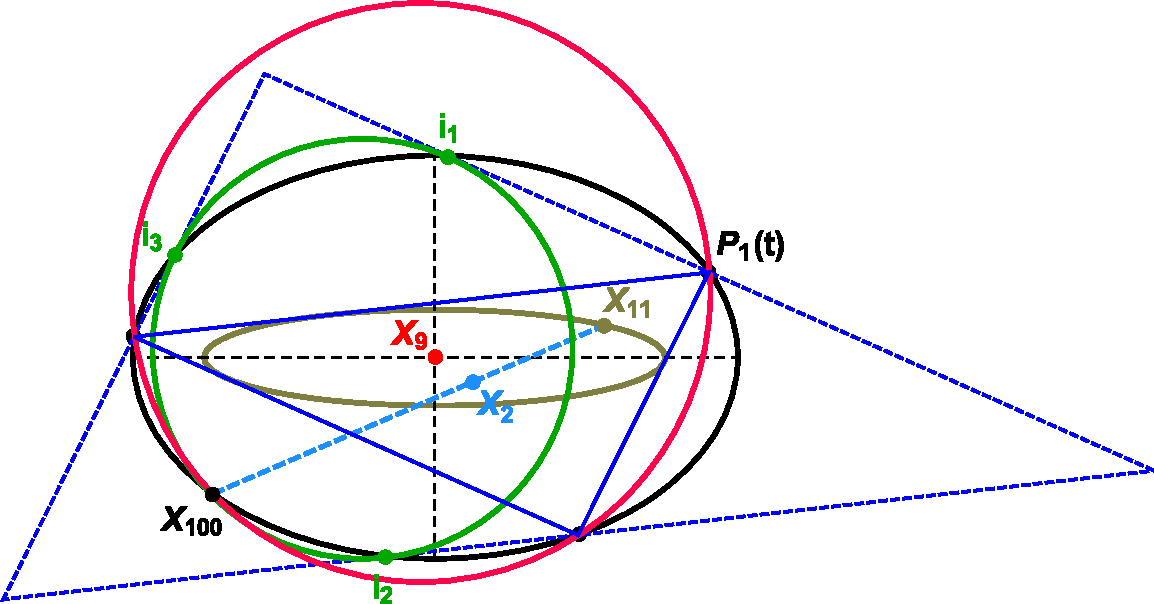
\includegraphics[width=\textwidth]{pics/0048_act_intouch.pdf}
    \caption{The locus of the three Intouch Points $i_1,i_2,i_3$ of the orbit's Anticomplementary Triangle (dashed blue) is the Billiard.}
    \label{fig:act_intouch}
\end{figure}

Furthermore, if $P_1(t)$ moves monotonically in one direction, the Anticomplementary's intouch points will move non-monotonically with respect to $P_1(t)$, Figure~\ref{fig:act-progress}. 

\begin{figure}[H]
    \centering
    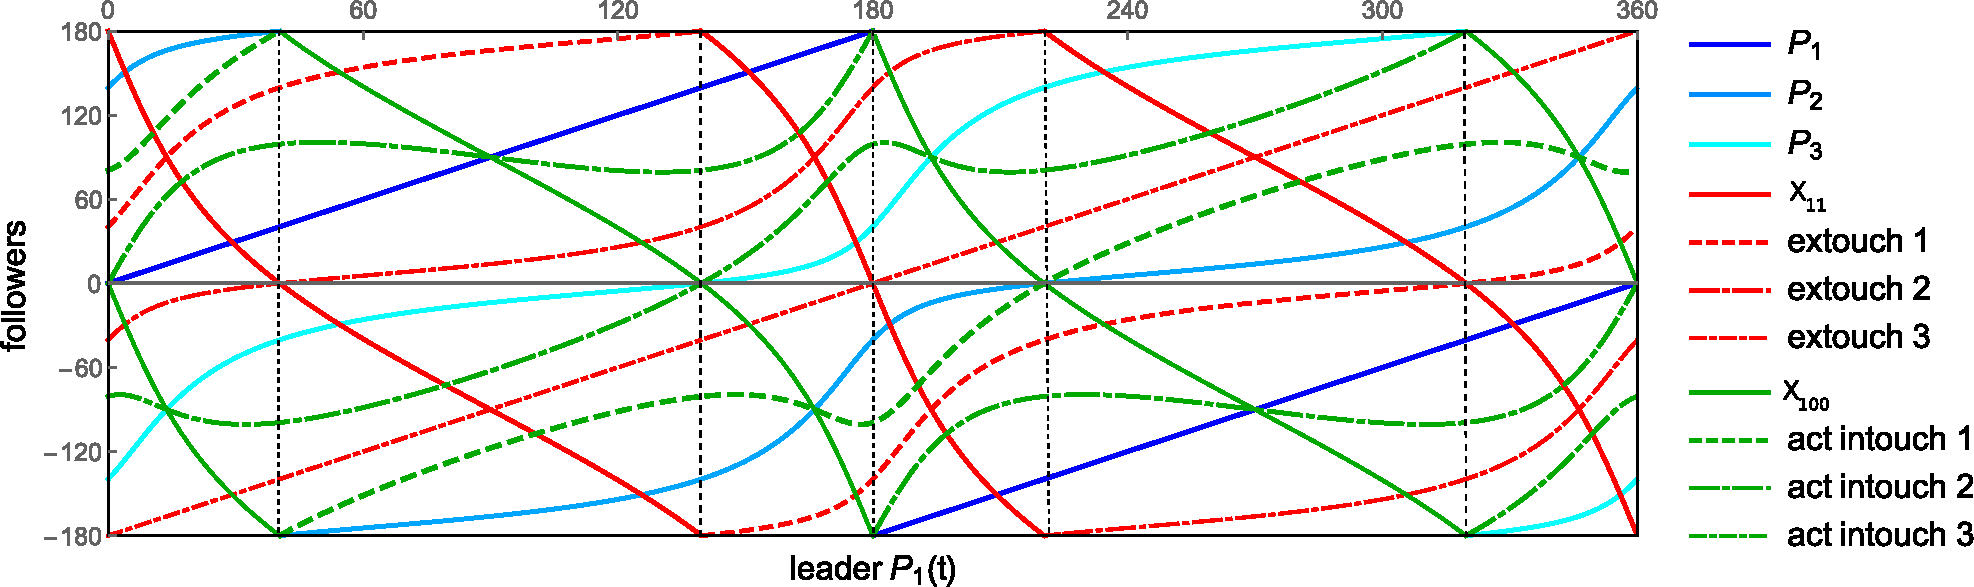
\includegraphics[width=\textwidth]{pics/0049_act_progress.pdf}
    \caption{Angular Progress along the Elliptic Billiard of (i) the $N=3$ orbit vertices $P_1(t)$ (black), $P_2,P_3$ (dark and light blue), (ii) the Feuerbach Point $X_{11}$ (red), always retrograde wrt. $P_1(t)$, (iii) the three Extouch Points (dashed reds) whose direction of motion is the same as $P_1(t)$, (iv) the Feuerbach Point of the Anticomplementary Triangle $X_{100}$ (green), moving opposite to $P_1(t)$, (v) the three Intouch Points of the Anticomplementary Triangle (dashed green), whose angular progress is non-monotonic with respect to $P_1(t)$.}
    \label{fig:act-progress}
\end{figure}
